%
% The first command in your LaTeX source must be the \documentclass command.
\documentclass[sigchi]{acmart}

%
% defining the \BibTeX command - from Oren Patashnik's original BibTeX documentation.
\def\BibTeX{{\rm B\kern-.05em{\sc i\kern-.025em b}\kern-.08emT\kern-.1667em\lower.7ex\hbox{E}\kern-.125emX}}
    
% Rights management information. 
% This information is sent to you when you complete the rights form.
% These commands have SAMPLE values in them; it is your responsibility as an author to replace
% the commands and values with those provided to you when you complete the rights form.
%
% These commands are for a PROCEEDINGS abstract or paper.
\copyrightyear{2019}
\acmYear{2019}
\setcopyright{acmlicensed}
\acmConference[SNA '19]{Social Network Analysis '19}{2018/19}{University of Pisa, Italy}
\acmBooktitle{Social Network Analysis '19}
\acmPrice{0.00}
%\acmDOI{10.1145/1122445.1122456}
%\acmISBN{978-1-4503-9999-9/18/06}


% end of the preamble, start of the body of the document source.
\begin{document}

%
% The "title" command has an optional parameter, allowing the author to define a "short title" to be used in page headers.
\title{Are you more “proukr” o “dontcare”? 
what a hashtag can say about you}

%
% The "author" command and its associated commands are used to define the authors and their affiliations.
% Of note is the shared affiliation of the first two authors, and the "authornote" and "authornotemark" commands
% used to denote shared contribution to the research.
\author{Davide Perra}
\email{d.perra@studenti.unipi.it}
\affiliation{%
  \institution{Student ID: 616686}
}

\author{Author 2}
\email{author.two@unipi.it}
\affiliation{%
  \institution{Student ID: 1234567}
}

\author{Author 3}
\email{author.three@unipi.it}
\affiliation{%
  \institution{Student ID: 1234567}
}


\renewcommand{\shortauthors}{One and Two, et al.}


% The abstract is a short summary of the work to be presented in the article.
\begin{abstract}
In this report, we propose a study conducted using Network Science tools regarding the relationships built up between users using the social network Twitter during the first weeks after the start of the war in Ukraine in February 2022.

\footnote{
{\bf Project Repositories}\\
\noindent Data Collection: \url{https://github.com/sna-unipi/data-collection}\\
\noindent Analytical Tasks: \url{https://github.com/sna-unipi/analytical-tasks}\\
\noindent Report: \url{https://github.com/sna-unipi/project-report}}
\end{abstract}


%
% Keywords. The author(s) should pick words that accurately describe the work being
% presented. Separate the keywords with commas.
\keywords{Social Network Analysis}


%
% This command processes the author and affiliation and title information and builds
% the first part of the formatted document.
\maketitle

\section{Introduction}
The outbreak of the Russian-Ukrainian conflict in February 2022 has been an important topic of discussion on social networks. Our analysis aims to construct a network inspired by the spread of the debate through the observation of tweets and retweets of users worldwide.
Within our network, nodes represent users and links represent interactions between them. We divided the nodes into 4 categories and the analysis carried out on the tweets and hashtags led us to analyse their trends with the ultimate goal of identifying what could be potential future scenarios within the network, in terms of the likelihood of a user changing their nature following an interaction with a user from a different category.


\section{Data Collection}
The first step was the data collection phase and the creation of a dataset. 
In order to set the work on data that best suited our needs, we decided to create a dataset by extracting data from Twitter to create our network. 


\subsection{Selected Data Sources}

We chose Twitter as the source for extrapolating the data as we believe it is one of the most widely used social networks for discussing the Russian-Ukrainian conflict as well as being, more generally, one of the most widely used platforms worldwide and thus able to engage a significant number of users. 
Although the official date of the outbreak of war is 24 February, we started analysing tweets from 15 February 2022 in order to capture users' opinions before the actual start date, until 15 March 2022, thus considering both the pre-war phase and the start phase, the highest moment that fragmented people's opinions. We use only one month for the network construction phase for reasons of memory management, performance, which were crucial considerations in the duration of the whole project due to the gigantic amount of tweets and related data and metadata. For the final phase of the open question, we enlarge the time view to two months.


\begin{itemize}
\item item 1
\item item 2
\item item 3
\end{itemize}

\subsubsection{Crawling Methodology and Assumptions}

{\bf Lorem ipsum dolor sit amet}, consectetur adipiscing elit, sed do eiusmod tempor incididunt ut labore et dolore magna aliqua. Ut enim ad minim veniam, quis nostrud exercitation ullamco laboris nisi ut aliquip ex ea commodo consequat. Duis aute irure dolor in reprehenderit in voluptate velit esse cillum dolore eu fugiat nulla pariatur. Excepteur sint occaecat cupidatat non proident, sunt in culpa qui officia deserunt mollit anim id est laborum\footnote{Duis aute irure dolor in reprehenderit in voluptate velit esse cillum dolore eu fugiat nulla pariatur \url{www.abcd.com}.}.

\begin{enumerate}
\item item 1
\item item 2
\item item 3
\end{enumerate}

\section{Network Characterization}

{\em Lorem ipsum dolor sit amet}, consectetur adipiscing elit, sed do eiusmod tempor incididunt ut labore et dolore magna aliqua. Ut enim ad minim veniam, quis nostrud exercitation ullamco laboris nisi ut aliquip ex ea commodo consequat. Duis aute irure dolor in reprehenderit in voluptate velit esse cillum dolore eu fugiat nulla pariatur. Excepteur sint occaecat cupidatat non proident, sunt in culpa qui officia deserunt mollit anim id est laborum.

\subsection{Comparision with ER}

Lorem ipsum dolor sit amet, consectetur adipiscing elit, sed do eiusmod tempor incididunt ut labore et dolore magna aliqua. Ut enim ad minim veniam, quis nostrud exercitation ullamco laboris nisi ut aliquip ex ea commodo consequat. Duis aute irure dolor in reprehenderit in voluptate velit esse cillum dolore eu fugiat nulla pariatur. Excepteur sint occaecat cupidatat non proident, sunt in culpa qui officia deserunt mollit anim id est laborum.

\subsection{Comparision with BA}

Lorem ipsum dolor sit amet, consectetur adipiscing elit, sed do eiusmod tempor incididunt ut labore et dolore magna aliqua. Ut enim ad minim veniam, quis nostrud exercitation ullamco laboris nisi ut aliquip ex ea commodo consequat. Duis aute irure dolor in reprehenderit in voluptate velit esse cillum dolore eu fugiat nulla pariatur. Excepteur sint occaecat cupidatat non proident, sunt in culpa qui officia deserunt mollit anim id est laborum.

\begin{equation}
  \lim_{n\rightarrow \infty}x= \sum_{i\in B]}\frac{1}{2}
\end{equation}




\section{Task 1: selected task}

Lorem ipsum dolor sit amet, consectetur adipiscing elit, sed do eiusmod tempor incididunt ut labore et dolore magna aliqua. Ut enim ad minim veniam, quis nostrud exercitation ullamco laboris nisi ut aliquip ex ea commodo consequat. Duis aute irure dolor in reprehenderit in voluptate velit esse cillum dolore eu fugiat nulla pariatur. Excepteur sint occaecat cupidatat non proident, sunt in culpa qui officia deserunt mollit anim id est laborum.

\begin{figure}[h]
  \centering
  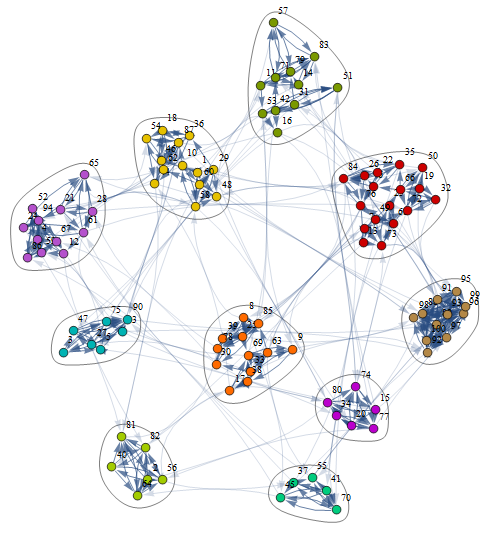
\includegraphics[width=\linewidth]{img/example_fig}
  \caption{Lorem ipsum dolor sit amet, consectetur adipiscing elit}
  \label{fig:example}
\end{figure}

Figure \ref{fig:example} as in \cite{lorem}.


\section{Task 2: selected task}

\begin{table}
  \caption{Excepteur sint occaecat cupidatat non proident}
  \label{tab:freq}
  \begin{tabular}{ccl}
    \toprule
    Col1 & Col2 & Col3\\
    \midrule
    A & B & C\\
    $\pi$ & D & E\\
    \$ & G & H\\
    $\Psi^2_1$ & I & L\\
  \bottomrule
\end{tabular}
\end{table}

Lorem ipsum dolor sit amet, consectetur adipiscing elit, sed do eiusmod tempor incididunt ut labore et dolore magna aliqua. Ut enim ad minim veniam, quis nostrud exercitation ullamco laboris nisi ut aliquip ex ea commodo consequat. Duis aute irure dolor in reprehenderit in voluptate velit esse cillum dolore eu fugiat nulla pariatur. Excepteur sint occaecat cupidatat non proident, sunt in culpa qui officia deserunt mollit anim id est laborum.

Table \ref{tab:freq}.

\section{Task 3: open question}

Lorem ipsum dolor sit amet, consectetur adipiscing elit, sed do eiusmod tempor incididunt ut labore et dolore magna aliqua. Ut enim ad minim veniam, quis nostrud exercitation ullamco laboris nisi ut aliquip ex ea commodo consequat. Duis aute irure dolor in reprehenderit in voluptate velit esse cillum dolore eu fugiat nulla pariatur. Excepteur sint occaecat cupidatat non proident, sunt in culpa qui officia deserunt mollit anim id est laborum.

\section{Discussion}

Lorem ipsum dolor sit amet, consectetur adipiscing elit, sed do eiusmod tempor incididunt ut labore et dolore magna aliqua. Ut enim ad minim veniam, quis nostrud exercitation ullamco laboris nisi ut aliquip ex ea commodo consequat. Duis aute irure dolor in reprehenderit in voluptate velit esse cillum dolore eu fugiat nulla pariatur. Excepteur sint occaecat cupidatat non proident, sunt in culpa qui officia deserunt mollit anim id est laborum.

% The next two lines define the bibliography style to be used, and the bibliography file.
\bibliographystyle{ACM-Reference-Format}
\bibliography{biblio}

\end{document}
